% Do not remove the next line
% Synchronized to r53967

\section {SSHD~- Secure-Shell, Secure-Copy}

Secure Shell offre la possibilité d'ajouter une connexion codée sur votre
routeur fli4l. De plus, avec la commande Secure Copy, vous pouvez transférer
des fichiers cryptés sur le routeur fli4l. Si à la connexion
\jump{SSHDPUBLICKEYN}{vous utilisez une clé publique}, vous pourrez alors
exécuter des commandes sur le routeur fli4l et transférer des fichiers script
qui pourront être exécutés. A partir de la version le 2.1.7 il a été rajouté
le serveur SSH2. 

\subsection {Installation du service Secure-shell}

\begin{description}

\config {OPT\_SSHD}{OPT\_SSHD}{OPTSSHD}

  Installation par défaut~: \var{OPT\_\-SSHD='no'}

  Si vous voulez accéder au routeur au moyen du ssh, il faut paramètrer la
  variable \var{OPT\_\-SSHD} sur \var{'yes'}. Cela installe un serveur-ssh
  dropbear sur le routeur fli4l. Cela permet également de copier les fichiers
  sur le routeur.

\config {SSHD\_ALLOWPASSWORDLOGIN}{SSHD\_ALLOWPASSWORDLOGIN}{SSHDALLOWPASSWORDLOGIN}

  Installation par défaut~: \var{SSHD\_ALLOWPASSWORDLOGIN='yes'}

  Si vous paramétrez la variable \var{SSHD\_ALLOWPASSWORDLOGIN} sur \var{'no'},
  la connexion ssh, avec un mot de passe au routeur fli4l, ne sera plus
  possible. Alors, la connexion au routeur se fera seulement au moyen
  d'une clé privée et d'une clé publique (key private/public). Cela suppose qu'une
  \jump{SSHDPUBLICKEYN}{clé publique} soit installée sur le routeur.

\config {SSHD\_CREATEHOSTKEYS}{SSHD\_CREATEHOSTKEYS}{SSHDCREATEHOSTKEYS}

  Installation par défaut~: \var{SSHD\_CREATEHOSTKEYS='no'}

  Le serveur-ssh a besoin d'une hostKey (ou clé d'hôte) qui doit être exceptionnelle
  et unique pour que le serveur-ssh s'identifie clairement au client-ssh. Certe
  le paquetage opt-sshd est fourni avec une hostKey, qui permet de se connecter pour
  la première fois au routeur fli4l avec le client-ssh, mais cette hostKey qui a
  été livrée doit être remplacée le plus vite possible, la hostKey sera remplacée
  et connu que par vous sont même. 
  Générer votre propre hostKey est important parce que c'est la seule manière
  possible de vous protéger contre les soi-disant Man-In-The-Middle-Attack.
  Votre client ssh peut remarquer, si un prétendu pirate est sur votre routeur
  fli4l, car le pirate ne connaît pas votre hostKey. Votre client ssh vous
  avertira par un message, si votre hostKey a été changé par le pirate.
 
  La création de votre hostKey (ou clé d'hôte) est entièrement automatique, une
  fois que le paramètre la variable \var{SSHD\_CREATEHOSTKEYS} est sur \var{'yes'}.
  Ce processus est très gourmand et peut prolonger, le temps du boot de plusieurs
  minutes. Si vous avez démarré le routeur fli4l avec l'activation de la variable
  \var{SSHD\_CREATEHOSTKEYS}, une (ou plusieurs) hostKey(s) sera produite dans
  le répertoire \var{/tmp/ssh}. Les fichiers produits à cet endroit, doivent
  être copié dans le répertoire, \var{etc/ssh} de votre sous-répertoire config
  (sur l'ordinateur donc vous avez créé le média de boot fli4l). Dans mon cas,
  voici l'arborescence du répertoire fli4l et le répertoire config.babel~:

  \begin{figure}[htbp]
    \centering
    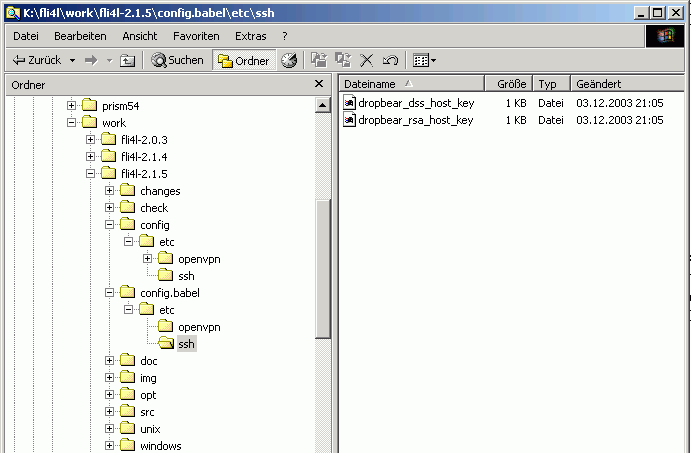
\includegraphics[width=\columnwidth]{etc_ssh_dir}
    \caption{Structure des répertoires fli4l}
    \label{fig:etc_ssh_dir}
  \end{figure}

  Faite attention, au sous-répertoire \var{config}, vous devez avoir le
  répertoire etc et le répertoire ssh. C'est précisément à cet endroit que la
  ou les hostKey(s) produite est copiée. A partir de la version 2.1.5 de fli4l,
  les fichiers de votre sous-répertoire config, sont prioritaire par rapport
  au sous-répertoire opt. Ainsi à la prochaine mise à jour de la version du
  routeur fli4l, les fichiers qui se trouvent dans le répertoire \var{config/etc/ssh}
  seront intégrés et non les fichiers qui se trouvent dans le répertoire
  \var{opt/etc/ssh}. Ainsi, il est possible pour chaque routeur fli4l d'utiliser
  ces propre hostKey. Lors de la construction des fichiers du routeur fli4l, un
  message apparaîtra à la fin, \flqq{}appending config specific files to
  opt.img ...\frqq{}. Alors, tous les fichiers venant du répertoire config
  seront listés et non les fichiers du répertoire opt.

\begin{verbatim}
#
# appending config specific files to opt.img ...
#
etc/ssh/dropbear_dss_host_key
etc/ssh/dropbear_rsa_host_key
\end{verbatim}

  Si vous avez produit une nouvelle clé d'hôte, remettez le paramètre de
  la variable \var{SSHD\_\-CREATEHOSTKEYS} sur \var{'no'}, de sorte que le
  script ne génère plus de nouvelle clé d'hôte à chaque démarrage du routeur fli4l.

  Après une mise à jour de votre routeur fli4l, si vous vous connectez au
  routeur, un message d'avertissement sera indiqué (différent selon le programme)
  par votre client ssh, qui attire l'attention sur un changement de votre hostKey.
  C'est normal, puisque vous venez justement de changer la hostKey, par celle
  fournie par fli4l. Suivez les instructions de votre client ssh, et modifié de
  façon permanente votre hostKey. Si vous recevez encore une fois ce message
  d'avertissement à une date ultérieure, vous devriez vérifier dans tous les
  cas, le pourquoi de cet avertissement, qui a été émis et non pas accepter
  aveuglément le changement de la hostKey. 

\begin{verbatim}
@@@@@@@@@@@@@@@@@@@@@@@@@@@@@@@@@@@@@@@@@@@@@@@@@@@@@@@@@@@
@    WARNING: REMOTE HOST IDENTIFICATION HAS CHANGED!     @
@@@@@@@@@@@@@@@@@@@@@@@@@@@@@@@@@@@@@@@@@@@@@@@@@@@@@@@@@@@
IT IS POSSIBLE THAT SOMEONE IS DOING SOMETHING NASTY!
Someone could be eavesdropping on you right now (man-in-the-middle attack)~!
It is also possible that the RSA host key has just been changed.
The fingerprint for the RSA key sent by the remote host is
ca:a4:ab:e7:af:d8:68:05:d3:1f:e6:15:08:d6:ed:36.
Please contact your system administrator.
Add correct host key in /home/babel/.ssh/known_hosts to get rid of this message.
Offending key in /home/babel/.ssh/known_hosts:7
Password authentication is disabled to avoid man-in-the-middle attacks.
\end{verbatim}

\config {SSHD\_PORT}{SSHD\_PORT}{SSHDPORT}

  Installation par défaut~: \var{SSHD\_PORT='22'}

  Avec la variable \var{SSHD\_PORT} vous pouvez indiquer un port différent
  du port par défaut sur lequel le serveur ssh doit fonctionner.

  Si vous voulez que l'on puisse accéder au ssh de l'extérieur, il faut 
  paramétrer la variable \jump{PFNEWCONFIG}{\var{INPUT\_ACCEPT\_PORT\_x}}

  Saisie des commandes pour utiliser le protocole SSH sur un ordinateur Unix
  ou Linux avec fli4l~:
  \begin{itemize}
  \item ssh~- Secure Shell
  \item scp~- Secure Copy
  \end{itemize}

  Les programmes pour Windows sont aussi disponibles~:
  \linebreak
  \altlink{http://www.chiark.greenend.org.uk/~sgtatham/putty/}
  \linebreak
  \altlink{http://winscp.net/eng/docs/lang:fr}
  \linebreak
  \altlink{http://www.tectia.com/en/en.iw3}

\config {SSHD\_PUBLIC\_KEY\_N}{SSHD\_PUBLIC\_KEY\_N}{SSHDPUBLICKEYN}

  Installation par défaut~: \var{SSHD\_PUBLIC\_KEY\_N='0'}

  Vous indiquez dans la variable \var{SSHD\_PUBLIC\_KEY\_N} le nombre de clés
  publiques qui doit être copié sur le routeur fli4l. 

  SSH permet l'authentification, à l'aide d'une procédures de cryptage asymétrique.
  Le contrôle d'authentification est utilisé avec une key Public/Privat à la
  place du nom d'utilisateur et du mot de passe. On s'épargner ainsi d'entrée
  d'un mot de passe. On produit la paire de clés à l'aide de keygen-ssh
  (ou puttygen, si on emploi putty sous Windows avec le client ssh). Optionnel
  une passphrase (ou phrase confidentielle) peut être indiqué pour une signature
  de la clé (on a besoin de ce mot de passe, si vous voulez utiliser la clé)
  cela augmente encore plus la sécurité. Si vous utilisez une passphrase vous
  devez réfléchir à l'utilisation d'un agent de clé (voir ssh-agent ou pageant).

  \wichtig{il y a deux clés, une clé publique et une clé privée, la clé privée,
  doit est traitée avec soin comme un mot de passe, puisqu'il remplit la même
  fonction. La clé privée est installée dans le client ssh. La clé publique est
  installée sur le routeur fli4l. Nous avons mis à disposition les variables
  suivant \var{SSHD\_PUBLIC\_KEY\_x} ou \var{SSHD\_PUBLIC\_KEYFILE\_x} pour
  gérer la clé publique.}

  Pour de plus amples informations, voir les pages du manuel ssh et ces composants,
  pour la documentation de putty voir
  (\altlink{http://www.chiark.greenend.org.uk/~sgtatham/putty/}).

\config {SSHD\_PUBLIC\_KEY\_x}{SSHD\_PUBLIC\_KEY\_x}{SSHDPUBLICKEYx}

  Dans cette variable vous pouvez indiquer la partie publique de la clé,
  pour l'utilisateur qui veut obtenir un accès ssh sur le routeur fli4l. Le
  plus simple pour récupérer la clé est d'utilisre le Cut-and-Paste (ou le
  couper-coller) à partir de la fenêtre du terminal. Cela pourrait par ex.
  ressembler à ceci~:

\begin{example}
\begin{verbatim}
        SSHD_PUBLIC_KEY_1='1024 ... username@hostname'
\end{verbatim}
\end{example}

 \wichtig{la clé ne contient pas de saut de ligne. Vous pouvez insérer les clés,
  produit par puttygen en externe, avec Cut-and-Paste (ou couper-coller). Cependant,
  les sauts de ligne doivent être supprimés.}

  Actuellement, les clés prises en charge pour les méthodes de chiffrement sont
  les suivantes~:
  \begin{itemize}
  \item DSA
  \item RSA
  \item ECDSA
  \end{itemize}

\config {SSHD\_PUBLIC\_KEYFILE\_N}{SSHD\_PUBLIC\_KEYFILE\_N}{SSHDPUBLICKEYFILEN}

  Installation par défaut~: \var{SSHD\_PUBLIC\_KEYFILE\_N='0'}

  Dans cette variable vous pouvez indiquer le nombre de fichiers Key. Au lieu de
  copier le contenu de la clé publique dans le fichier sshd.txt, vous pouvez
  copier la clé publique directement dans l'archive-opt. Cela fonctionne comme
  la variable \var{SSH\_CREATEHOSTKEYS} décrit plus haut. Copiez votre clé
  publique dans un fichier et placez-le dans le répertoire \var{$<$config$>$/etc/ssh}.

\config {SSHD\_PUBLIC\_KEYFILE\_x}{SSHD\_PUBLIC\_KEYFILE\_x}{SSHDPUBLICKEYFILEx}

  Dans cette variable vous pouvez indiquer le nom du fichier de la clé publique
  que vous avez enregistré dans répertoire \var{$<$config$>$/etc/ssh}.

\begin{example}
\begin{verbatim}
        SSHD_PUBLIC_KEYFILE_1='root@fli4l'
\end{verbatim}
\end{example}

  Actuellement, les clés prises en charge pour les méthodes de chiffrement sont
  les suivantes~:
  \begin{itemize}
  \item DSA
  \item RSA
  \item ECDSA
  \end{itemize}

\config {SSH\_CLIENT\_PRIVATE\_KEYFILE\_N}{SSH\_CLIENT\_PRIVATE\_KEYFILE\_N}{SSHCLIENTPRIVATEKEYFILEN}

  Installation par défaut~: \var{SSH\_CLIENT\_PRIVATE\_KEYFILE\_N='0'}

  Dans cette variable vous pouvez indiquer le nombre de fichiers Key. Si la clé
  privée est compatible avec le client ssh ou plink pour une connexion à un serveur
  SSH désiré, vous pouvez copier cette dernière dans le répertoire \var{$<$config$>$/etc/ssh}.
  Cela fonctionne comme la variable \var{SSH\_CREATEHOSTKEYS} décrit plus haut. 
  Si vous avez copié votre clé privée dans le répertoire \var{$<$config$>$/etc/ssh}.
  La clé privée au format OpenSSH sera convertie automatiquement à chaque processus
  de départ de fli4l au format dropbear.

\config {SSH\_CLIENT\_PRIVATE\_KEYFILE\_x}{SSH\_CLIENT\_PRIVATE\_KEYFILE\_x}{SSHCLIENTPRIVATEKEYFILEx}

  Dans cette variable vous pouvez indiquer le nom du fichier de la clé publique
  que vous avez enregistré dans le répertoire \var{$<$config$>$/etc/ssh}.

\begin{example}
\begin{verbatim}
        SSHD_PRIVATE_KEYFILE_1='babel@rootserver'
\end{verbatim}
\end{example}

  Actuellement, les clés prises en charge pour les méthodes de chiffrement sont
  les suivantes~:
  \begin{itemize}
  \item DSA
  \item RSA
  \item ECDSA
  \end{itemize}

\end{description}

\subsection {Installation du dbclient}

\begin{description}

\config {OPT\_SSH\_CLIENT}{OPT\_SSH\_CLIENT}{OPTSSHCLIENT}

  Installation par défaut~: \var{OPT\_SSH\_CLIENT='no'}

  Si vous voulez utiliser un authentique client ssh2, vous pouvez activer dbclient
  dropbear en paramétrant la variable sur \var{OPT\_SSH\_CLIENT='yes'}. Ce client
  a l'avantage de partager de nombreux programmes codés, avec le serveur ssh
  dropbear. Vous pouvez ainsi épargner de la place dans l'archive-OPT. Le dbclient est
  compatible avec de nombreux client ssh/scp, de plus, les paramètres de commandes
  sont semblables. Il y a également un lien symbolique créé vers /usr/bin/ssh, alors
  cela fonctionne habituellement avec ssh $<$host$>$ ou scp $<$source$>$ $<$target$>$.

  Si vous voulez sauvegarder la clé d'hôte du dbclient de façon permanente,
  vous devez copier le fichier known\_hosts du répertoire /.ssh sur le
  routeur fli4l, dans le répertoire config/etc/ssh. Cela se passe comme
  si l'on produisait une clé d'hôte. Dans l'exemple suivant le dépaquetage fli4l
  se trouve dans le répertoire (dans le quel le support de boot fli4l est créée)
  /home/babel/fli4l-\version~ . Tous les fichiers de configuration se trouvent
  dans le répertoire config.babel.

\begin{example}
\begin{verse}
\texttt{cd /home/babel/fli4l-\version}\\
\texttt{mkdir -p config.babel/etc/ssh}\\
\texttt{scp fli4l:/.ssh/* config.babel/etc/ssh}
\end{verse}
\end{example}

\end{description}

\subsection {Installation du client plink}

\begin{description}

\config {OPT\_PLINK\_CLIENT}{OPT\_PLINK\_CLIENT}{OPTPLINKCLIENT}

  Installation par défaut~: \var{OPT\_PLINK\_CLIENT='no'}

  Installer sur le routeur fli4l le client ssh1/ssh2/telnet. Le programme plink
  est la version Unix, du programme PuTTY connu sous Windows. Un appel de plink
  sur le routeur fli4l affiche la page d'aide, pour l'utilisation de plink.

  Si vous voulez sauvegarder la hostKey (ou clé d'hôte) dans plink, de façon
  permanente, vous devez copier le fichier sshhostkeys à partir du répertoire
  /.putty sur le routeur fli4l, il doit être copier dans le répertoire config/etc/plink.
  Cela se passe comme si l'on produisait une hostKey. Dans l'exemple suivant le
  dépaquetage de fli4l se trouve dans le répertoire (dans le quel le support de
  boot fli4l est produite /home/babel/fli4l-\version~ . Tous les fichiers de
  configuration se trouvent dans le répertoire config.babel.

\begin{example}
\begin{verse}
\texttt{cd /home/babel/fli4l-\version}\\
\texttt{mkdir -p config.babel/etc/plink}\\
\texttt{scp fli4l:/.putty/* config.babel/etc/plink}
\end{verse}
\end{example}

\end{description}

\subsection {Installation d'un serveur sftp}

\begin{description}

\config {OPT\_SFTPSERVER}{OPT\_SFTPSERVER}{OPTSFTPSERVER}

  Installation par défaut~: \var{OPT\_SFTPSERVER='no'}

  Installe sur le routeur fli4l un serveur-sftp.

\end{description}

\subsection{Littérature}

Site Web de Dropbear SSH2~: \altlink{http://matt.ucc.asn.au/dropbear/dropbear.html}

Première version de la documentation par
Claas Hilbrecht $<$babel@fli4l.de$>$, Avril 2004
